\section{Design and Implementation}\label{sec:design}

\subsection{Overview of Workflow and System Components}\label{sec:hector_overview}
Hector consists of a programming interface, a code generator, and Python modules.
The code generator takes in the model definition and generates both CUDA kernels and host functions that configure and invoke the CUDA kernels.


\begin{figure}[!t]
\centering
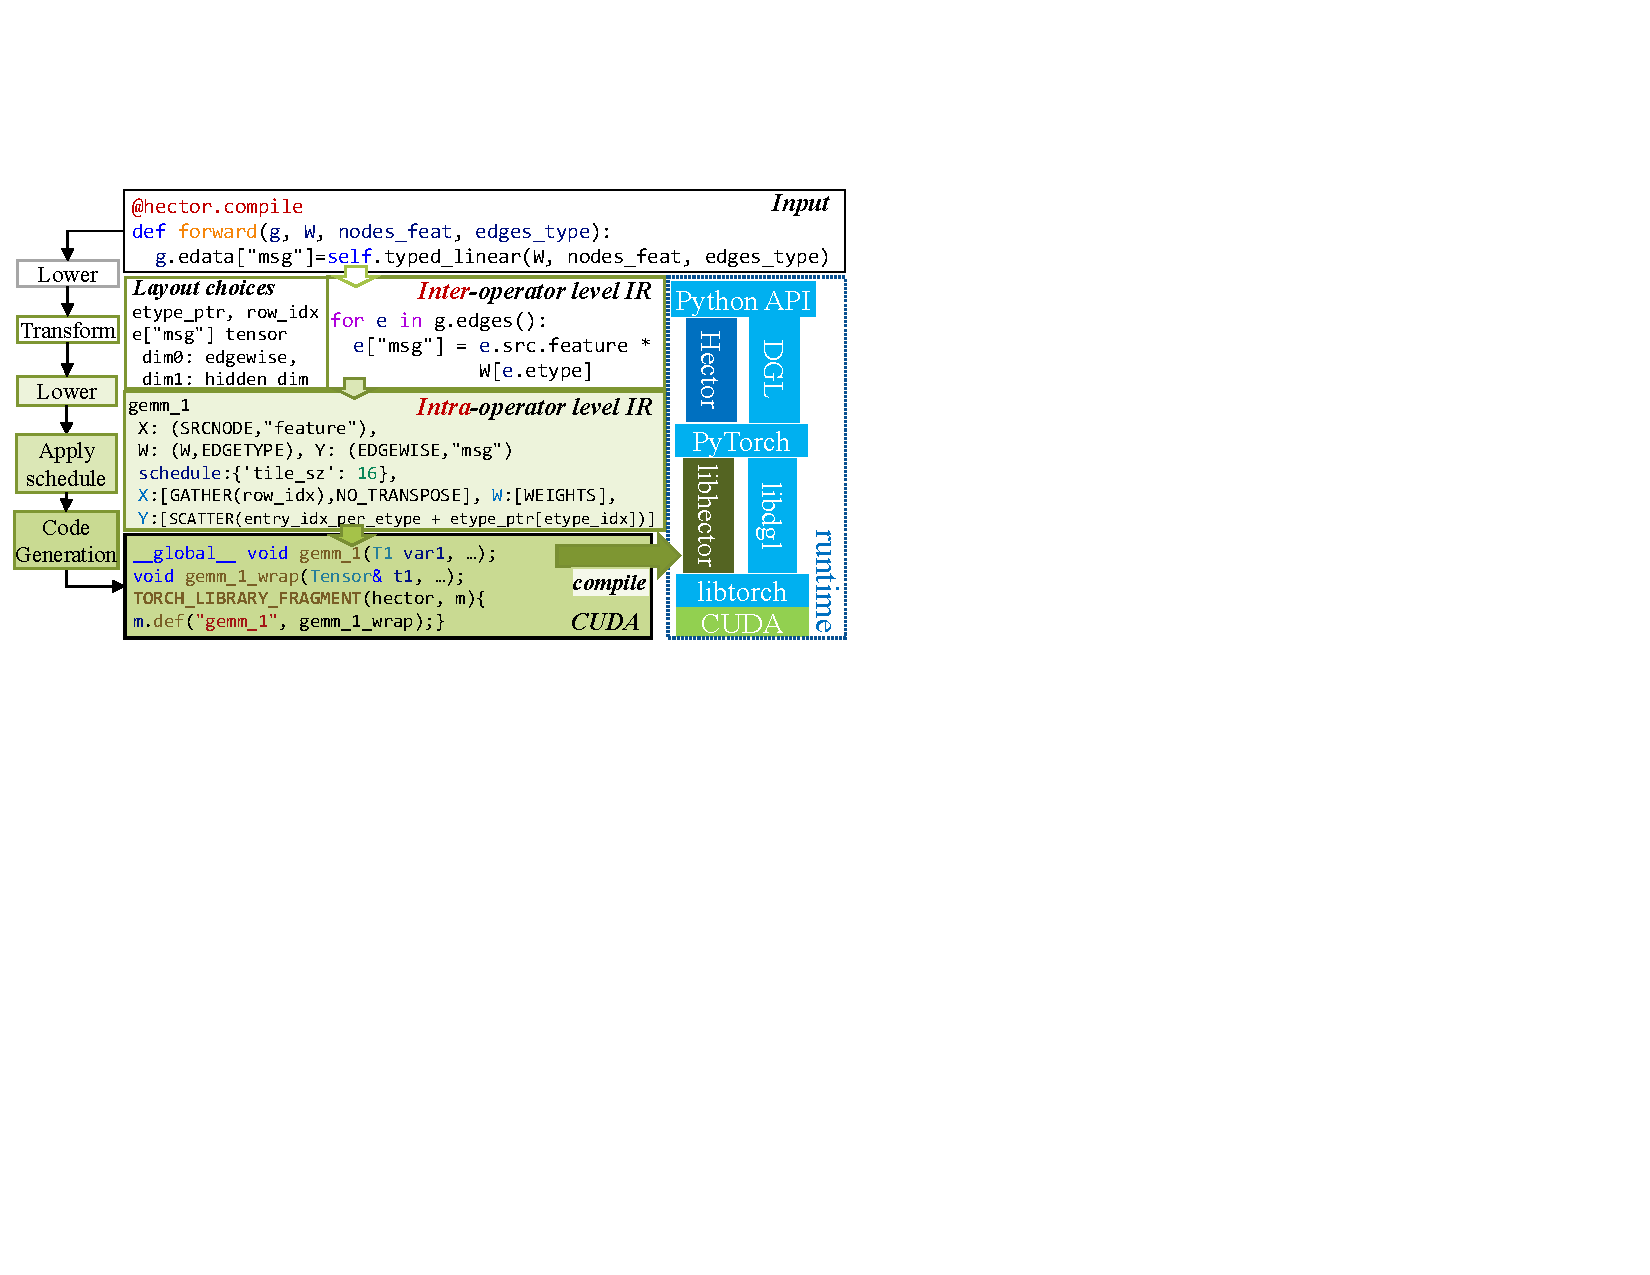
\includegraphics[width=\linewidth]{figures/Hector/RuntimeArch_v3.6.pdf}
\caption{\label{fig:runtime_arch} Hector workflow and software architecture. }
\end{figure}


Figure~\ref{fig:runtime_arch} uses an example to illustrate the workflow. The input is an excerpt of DGL code invoking a typed linear layer on the input node features. Applying the \texttt{@hector.compile} decorator triggers a transpiling pass to lower the code into Hector inter-operator level IR. {In this example, the typed linear transformation \texttt{typed\_linear}} can be efficiently implemented as GEMM kernels. {To this end,} Hector lowers the transform to an operator instance derived from the GEMM template at the inter-operator level. {After the analysis and optimizations at the inter-operator level, Hector further lowers the code to a detailed GEMM specification at the intra-operator level.} The GEMM output $A$ collects edge data generated from the node data. The first input $B$ is the weight matrix $W$, and the second input $C$ is the collection of features of all the source nodes of the edges involved. The intra-operator level IR indicates that the GEMM operation should use the default tile width of 16 and be carried out without scatter, gather, or transpose applied to input or output matrices. Eventually, Hector generates a segment MM~(Section~\ref{sec:segmentmm}) kernel, \texttt{gemm\_1}. 
The Layout Choices section of Figure~\ref{fig:runtime_arch} shows the default layout choice. \texttt{etype\_ptr} specifies the offsets of each segment of different type. \texttt{row\_idx} is the source node index array in the COO format. The result tensor \texttt{e["msg"]} has the number of edges as the number of rows, and the number of the columns is the input dimension of the hidden layer. We detail in Section~\ref{sec:materialization} an optimization technique, compact materialization, that is opened up by the decoupled layout choices from the inter-operator level IR.




The generated code is compiled into a shared library where host functions are exported through the \texttt{pybind11} utilities.
Hector falls back to existing routines in PyTorch when certain operators are not yet supported.
During runtime, the precompiled functions are loaded and registered as subclasses of PyTorch \texttt{autograd.Function}.












\subsection{Inter-Operator Level IR}
\label{sec:inter_op_ir}

The inter-operator level IR follows the Python grammar but involves some new constructs, as listed in Table~\ref{tab:ir_constructs}. Listing~\ref{lst:ir_example} illustrates how the attention calculation in a single-headed RGAT layer could be expressed using the inter-operator level IR.
Lines 10-16 shows a code segment that generates attention values for all edges of graph \texttt{g} and then invoke the \texttt{edge\_softmax(g)} function that spans lines 1 through 9. As shown in Listing~\ref{lst:ir_example}, the message generation and aggregation stages are expressed as for-each edge loops starting from line~2, line~8, and line~10, and for-each node loop starting from line~4. To accumulate data from the incoming edges of each node n, the \texttt{n.incoming\_edges()} iterator is used. Notably, the data layout that specifies how to access the input and output data per edge or node as well as the incoming edges associated with each node, is abstracted away in Listing~\ref{lst:ir_example}.



\subsubsection{Programming Interface}
Hector provides a decorator, \texttt{@hector.compile}, to take the existing PyG or DGL forward propagation logic and generate code for it, as exemplified by the input in Figure~\ref{fig:runtime_arch}. The decorator, when applied to a method, invokes a simple transpiling pass that replaces the PyG and DGL method calls, e.g., SpMM/SDDMM,  with an implementation in the inter-operator level IR, and replaces supported constructs from PyG and DGL with expressions in Hector IR.
Similarly to statically-typed compilers in other Python packages~\cite{pytorchTorchScriptPyTorchDocumentation, lamNumbaLLVMbasedPython2015}, the function to compile can use most of the Python features except dynamic ones, e.g., assigning objects of different types to the same variable. We support a few types as the function arguments for heterogeneous graphs, involving \texttt{Tensor} and \texttt{dict[str, Tensor]} objects, i.e., \texttt{dict} objects where the keys are \texttt{str} objects and the values are \texttt{Tensor} objects.

Besides, one can use the Hector inter-operator level IR itself to express the model, as exemplified by Listing~\ref{lst:ir_example}. %


\begin{lstlisting}[caption={Expressing the attention calculation in a single-headed RGAT model using Hector inter-operator level IR.},label={lst:ir_example},language=Python]
def edge_softmax(g):
    for e in g.edges():
        e["att"] = exp(e["att"])
    for n in g.dst_nodes():
        n["att_sum"] = 0.0
        for e in n.incoming_edges():
            n["att_sum"] += e["att"]
    for e in g.edges():
        e["att"] /= e.dst["att_sum"]
for e in g.edges():
    hs = e.src.feature * W[e.etype]
    atts = dot_prd(hs, w_s[e.etype])
    ht = e.dst.feature * W[e.etype]
    attt = dot_prd(ht, w_t[e.etype])  
    e["att"] = leakyrelu(atts + attt)
edge_softmax(g)
\end{lstlisting}


\begin{figure}[!htbp]
\centering
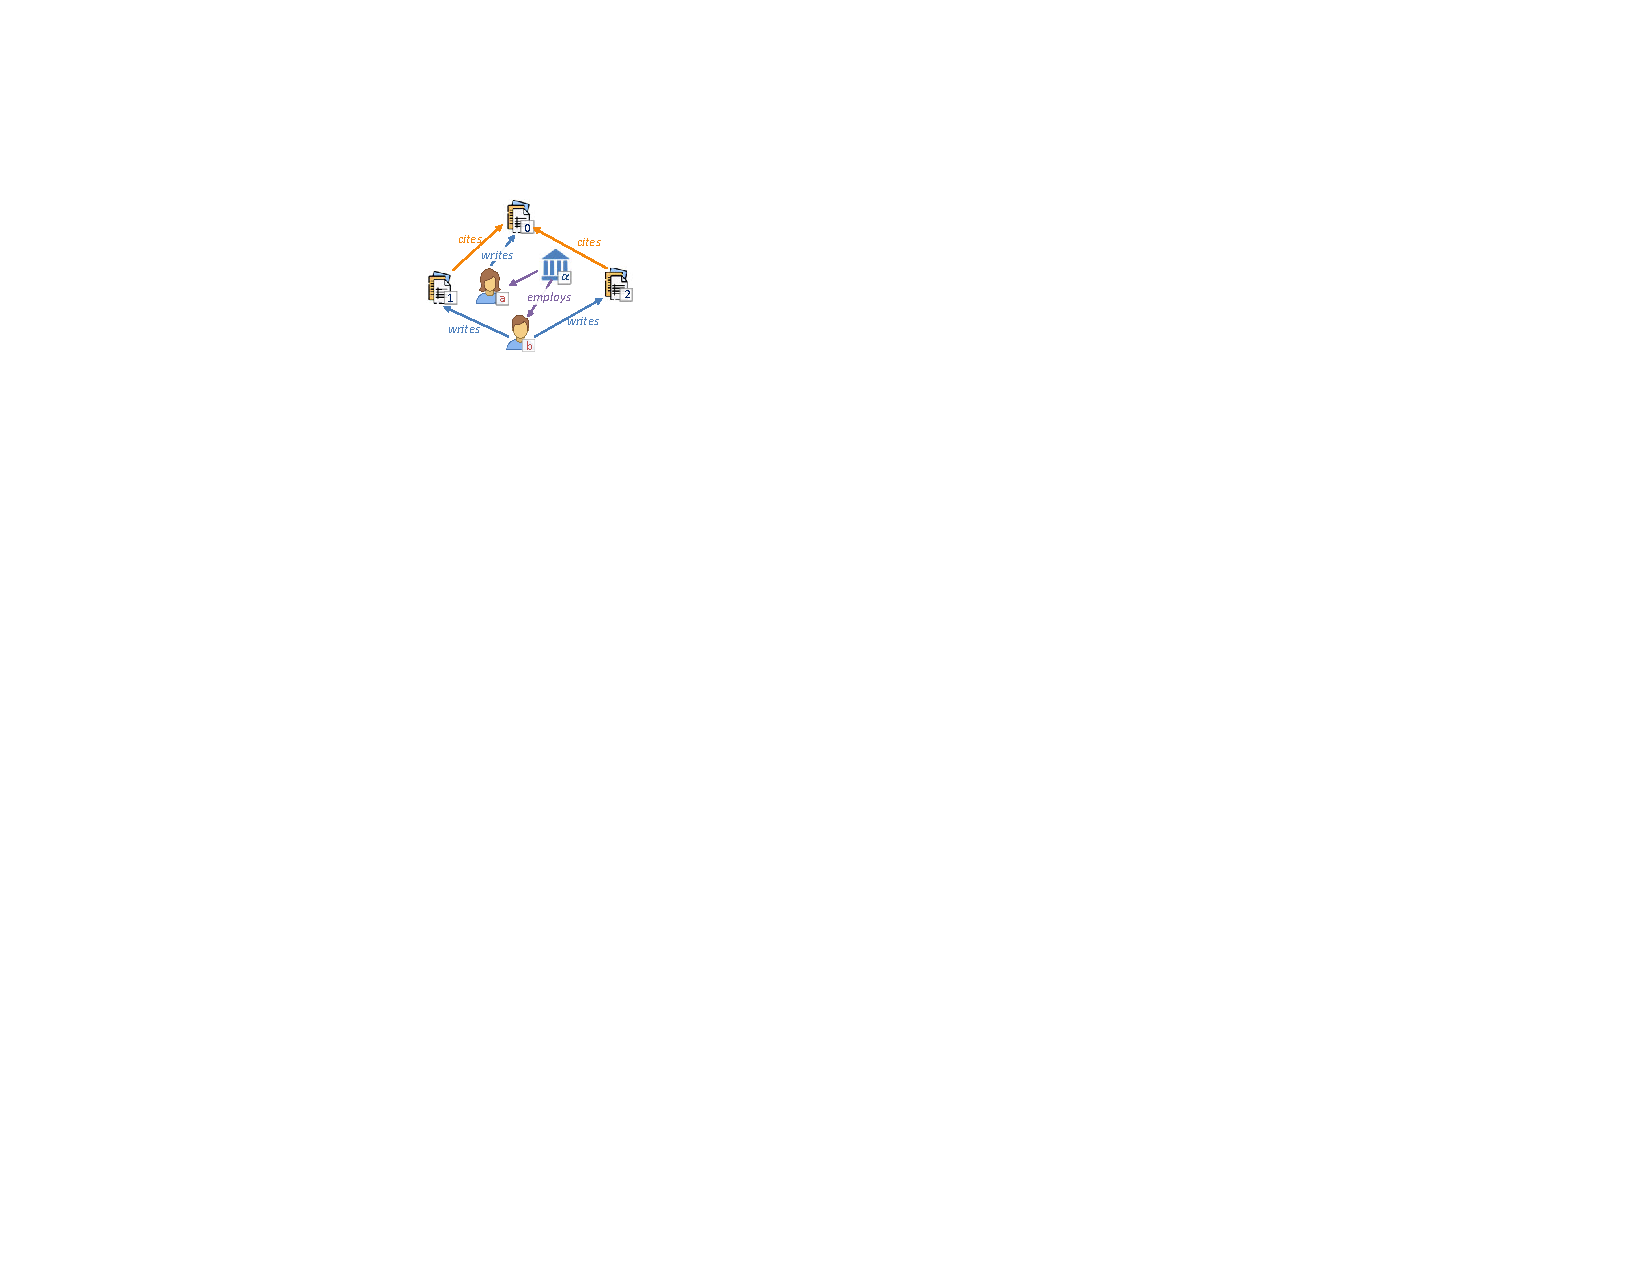
\includegraphics[width=0.4\linewidth]{figures/Hector/supplemental_opt_example.pdf}
\caption{\label{fig:opt_example} The citation graph used as the example in Figures~\ref{fig:compact_opt_opt}~and~\ref{fig:linear_opt}. }
\end{figure}

\begin{figure}[!htbp]\captionsetup[subfigure]{font=small}
\centering
\subcaptionbox{GEMM kernel and IRs of RGAT edge message computation with vanilla materialization. The two red squares mark identical terms because \texttt{msg} depends only on source node and edge type. Both schemes in (a) and (b) \textcircled{1} gather the source node’s features into a matrix, \textcircled{2} perform the GEMM computation, and \textcircled{3} scatter the output features to rows in the output tensor. Each dotted square mark a block in \textcircled{2} the GEMM kernel. \texttt{row\_idx} specifies the source node index of each edge, and is used in step \textcircled{1}. \texttt{etype\_ptr} specifies the offsets of edge of each type and is used in step \textcircled{3}.}
[\linewidth]{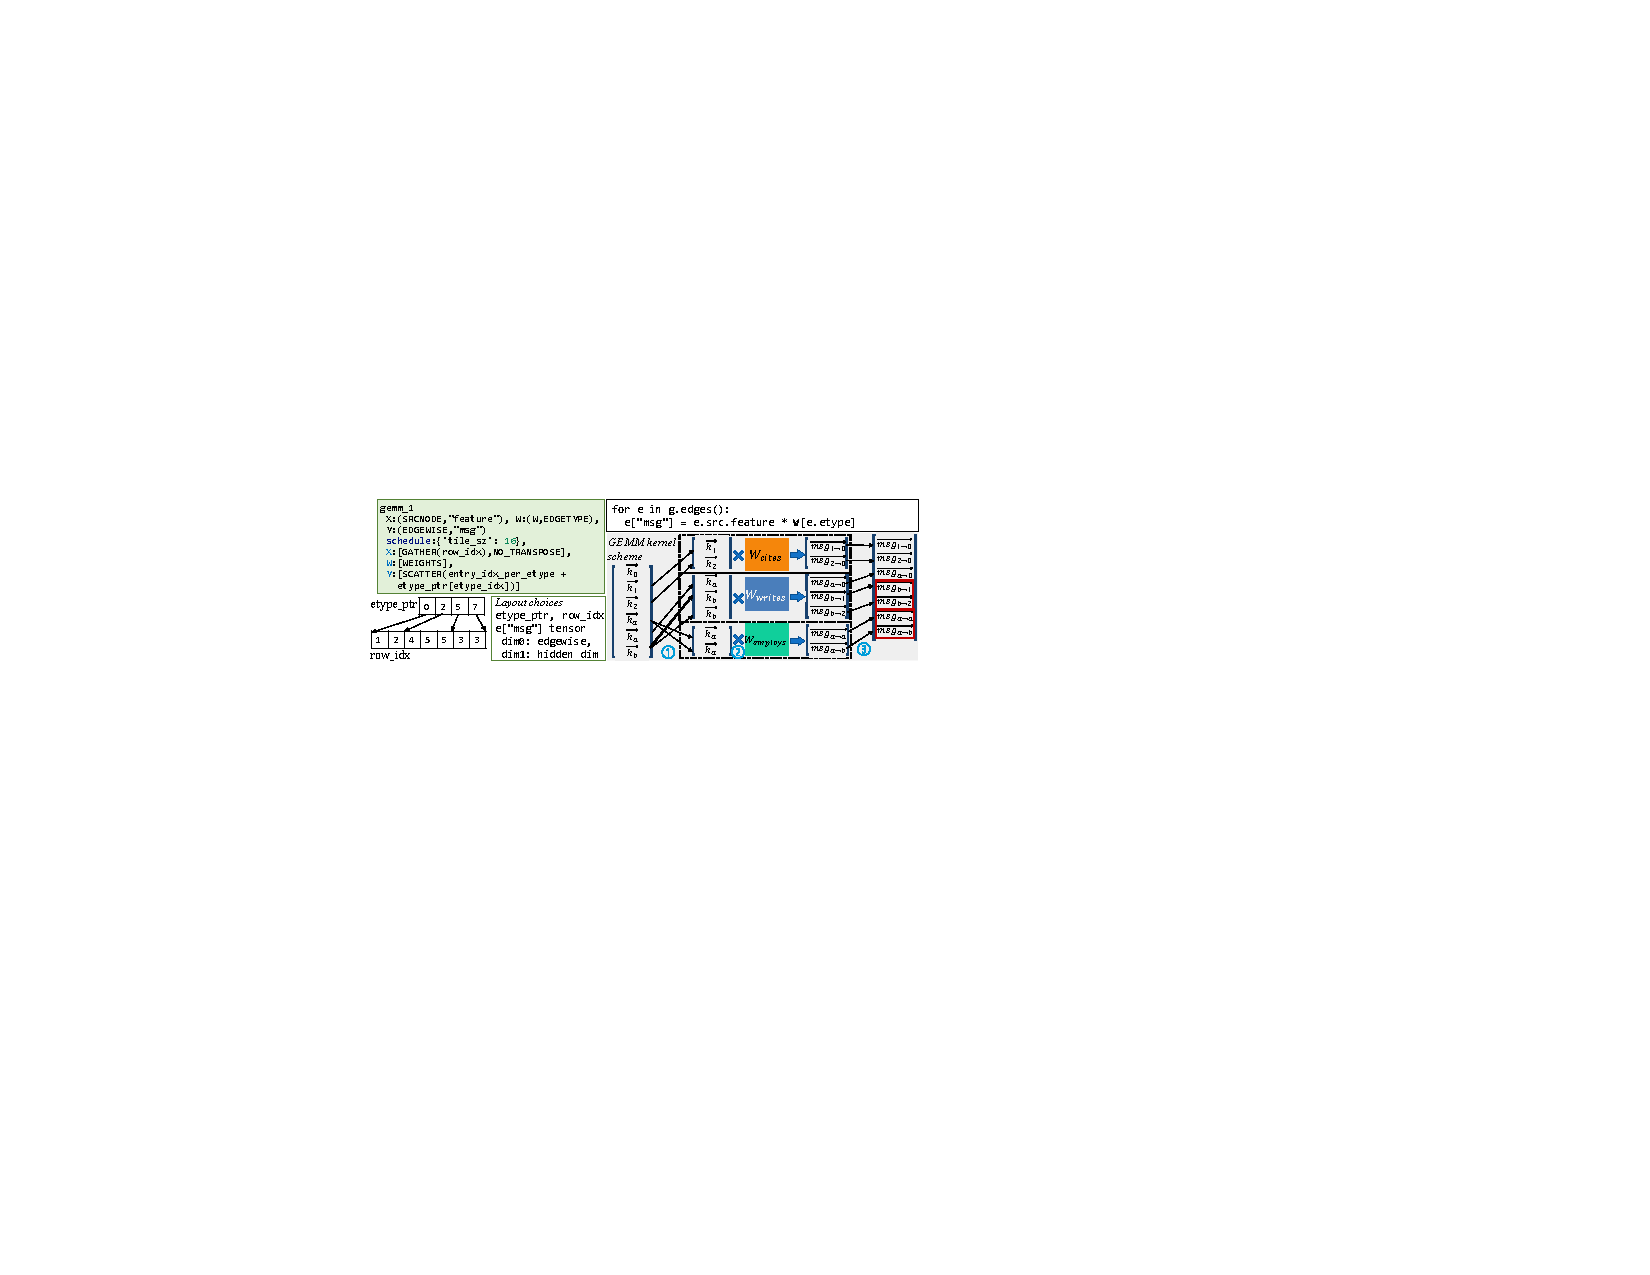
\includegraphics[scale=1.47]{figures/Hector/supplemental_compact.final.up.pdf}}
\subcaptionbox{GEMM kernel and IRs of RGAT edge message computation with compact materialization. Differences in IRs are marked in orange.}
[\linewidth]{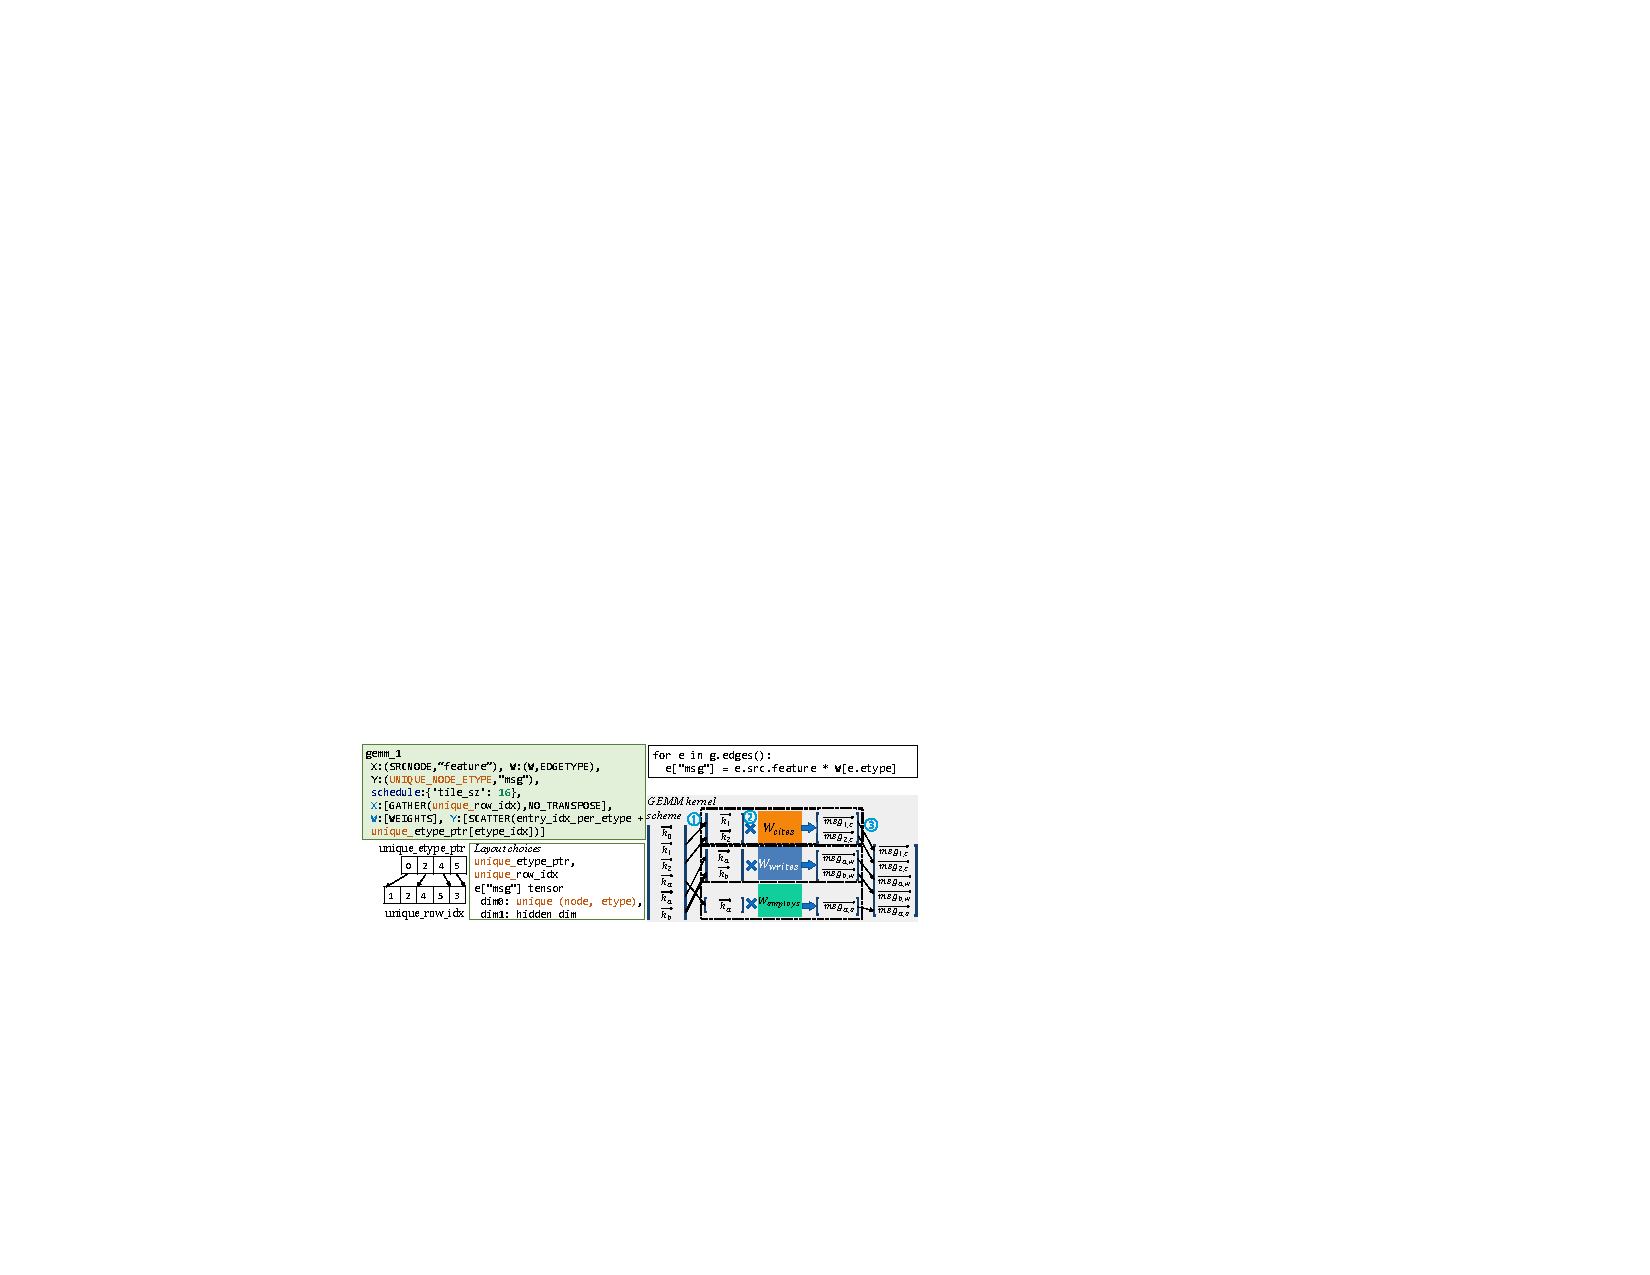
\includegraphics[scale=1.45]{figures/Hector/supplemental_compact.final.down.pdf}}
\caption{\label{fig:compact_opt_opt} When computing RGAT edge messages, compact materialization could be applied. This figure uses the graph in Figure~\ref{fig:opt_example}. Compared with (a)~vanilla materialization, (b)~compact materialization saves both the memory footprint and the computation. In (a), the leading dimension of the output message tensor accommodates different edges. In (b), it accommodates unique (source node, edge type) pairs. \texttt{unique\_row\_idx}, and \texttt{unique\_etype\_ptr} describes the mapping from (source node index, edge type index) to the unique index.}
\end{figure}

\subsubsection{Compact Tensor Materialization and Data Layout}
\label{sec:materialization}

{The} Hector inter-operator level IR deliberately abstracts away the data layout from the model semantics. As exemplified by Listing~\ref{lst:ir_example}, the IR only expresses the association of variables with nodes or edges, e.g., \texttt{e["att"]} and \texttt{n["att\_sum"]}, without dictating the mapping of elements in the conceptual variable to the memory space. 

In Hector, we devised compact materialization, which is a technique enabled by the decoupling between model semantics and data layout. 
Note that certain edge data are determined by sparse combinations of source node features and edge types, e.g.  $\overrightarrow{{msg}_{HGT}}$ in Figure~\ref{fig:rgat_layer}. Rather than computing and storing such data for each edge, we instead compute and store the data once for each $\left(\text{edge type}, \text{unique node index}\right)$ pair  that actually exists, reducing the resources spent on computing and storing common subexpressions.
As exemplified in Figure~\ref{fig:compact_opt_opt}, the materialized tensor involves seven rows when each row vector corresponds to a \texttt{msg} of an edge.
Alternatively, the system can materialize the tensor with only five rows, where each row vector corresponds to a \texttt{msg} of an $\left(\text{edge type}, \text{unique node index}\right)$ pair.
We call the former vanilla materialization and the latter compact materialization.
For the vanilla scheme, the row number is the edge index specified by the sparse adjacency. For the compact scheme, it is a unique non-negative integer assigned to each $(\text{source node}, \text{edge type})$. We precompute this mapping and store it in a CSR-like format. Hector does not create the temporary weight tensor, as explained in Section~\ref{sec:segmentmm}.
In summary, compact materialization is a technique to eliminate repetitive identical computations and results in edgewise operators. It is applicable when an edgewise operator depends only on the source node data and edge type, and its output has the shape of $(\text{number of edges}, \text{hidden dimension size})$. After this optimization, the output shape is reduced to $(\text{number of unique} \allowbreak (source\ \allowbreak node, edge\ type)\text{ pairs}, \text{hidden dimension size})$, and repetitive computation is eliminated.
Section~\ref{sec:dse_eval} provided further analysis of the effects of compact materialization on memory footprint reduction.


\begin{table}[!htbp]
\centering
\begin{tabular}{@{}l@{}l@{}l@{}l@{}}
\multicolumn{4}{l}{\textbf{Methods of graph variables}}\\\hline
\multicolumn{1}{|l}{node iterator}        & \multicolumn{3}{l|}{\texttt{g.dst\_nodes()}, \texttt{g.src\_nodes()}}                                                      \\\hline
\multicolumn{4}{|l|}{
\noindent{
\begin{tabular}[t]{@{}ll|ll@{}}
\hspace{-2.25pt}edge iterator        & \texttt{g.edges()}  & weight slicing, e.g.,    &\texttt{W[e.etype]} \\
\end{tabular}}}     \\\hline
\multicolumn{1}{|l}{neighbor iterator}    & \multicolumn{3}{l|}{\texttt{n.incoming\_edges()}, \texttt{n.outgoing\_edges()}}\\\hline 
\multicolumn{4}{l}{\rule{0pt}{10pt}\textbf{Attributes}}\\\hline
\multicolumn{4}{|l|}{
\noindent{
\begin{tabular}[t]{@{}ll|ll@{}}
\hspace{-2.25pt}nodes                & \texttt{e.src}, \texttt{e.dst}                       & types                       & \texttt{e.etype}, \texttt{n.ntype}  
\end{tabular}}}     \\\hline
\multicolumn{4}{|l|}{
\noindent{
\begin{tabular}[t]{@{}ll|ll@{}}
\hspace{-2.25pt}input data, e.g.,    & \texttt{n.feature}      &produced data, e.g.,& \texttt{e["att"]}
\end{tabular}}}     \\\hline
\multicolumn{4}{l}{\rule{0pt}{10pt}\textbf{Operators}}\\\hline
\multicolumn{2}{|l}{GEMM-eligible computation, e.g.,}        & \multicolumn{2}{l|}{\texttt{linear()}, \texttt{outer\_prod()}}                                                      \\\hline
\multicolumn{2}{|l}{GEMM-ineligible computation, e.g.,}    & \multicolumn{2}{l|}{\texttt{dot\_prod()}} \\\hline
\multicolumn{2}{|l}{manipulation, e.g.,}    & \multicolumn{2}{l|}{\texttt{reshape()}, \texttt{concat()}} \\\hline
\end{tabular}
\caption{Hector inter-operator level IR constructs. The graph's variable is named as \texttt{g}, node's as \texttt{n}, and edge's as \texttt{e}. }\label{tab:ir_constructs}
\end{table}


Besides tensor materialization, the multi-level IR design also allows data layout optimizations involving 1)~architecture-specific optimizations, e.g., padding, and 2)~various sparse adjacency encoding.
At the inter-operator level, data layout specifications are decoupled from the model semantics and do not influence the transform passes at this level. 
However, they determine the data access scheme and make a difference when generating CUDA code at the intra-operator level.
Hector inter-operator level IR bookkeeps the specifications, which are passed to the intra-operator level during lowering. 
The intra-operator level operator instances choose the data access scheme corresponding to the data layout specifications while assembling the kernel code.
We leave the exploration of data layout optimizations to future work and detail our plan in Section~\ref{sec:future_work}. 




\subsubsection{Linear Operator Reordering}
\label{sec:inter_op_opt}
Linear operator reordering is an inter-operator level optimization. When a linear operator, e.g., linear layer and dot product, is followed by another linear operator, their order may be switched. 
For example, for \texttt{atts} as shown in Figure~\ref{fig:linear_opt}(c), we may calculate $W_r\vec{w}_{r}^T$ first instead. Its profitability can be determined by counting the number of multiplication and addition involved in the two GEMMs before and after the order is changed. For now, we implement the pass to switch the orders of two linear operators whenever this produces an operator between weights, because it reduces the complexity by reducing one of its factors, the number of nodes/edges, to the size of hidden dimension. For simplicity, rewritten operator instances use PyTorch BMM to compute the product of weights and apply PyTorch slicing when necessary.


\begin{figure}[!htbp]\captionsetup[subfigure]{font=small}
\centering
\subcaptionbox{The original inter-operator level IR.}
[\linewidth]{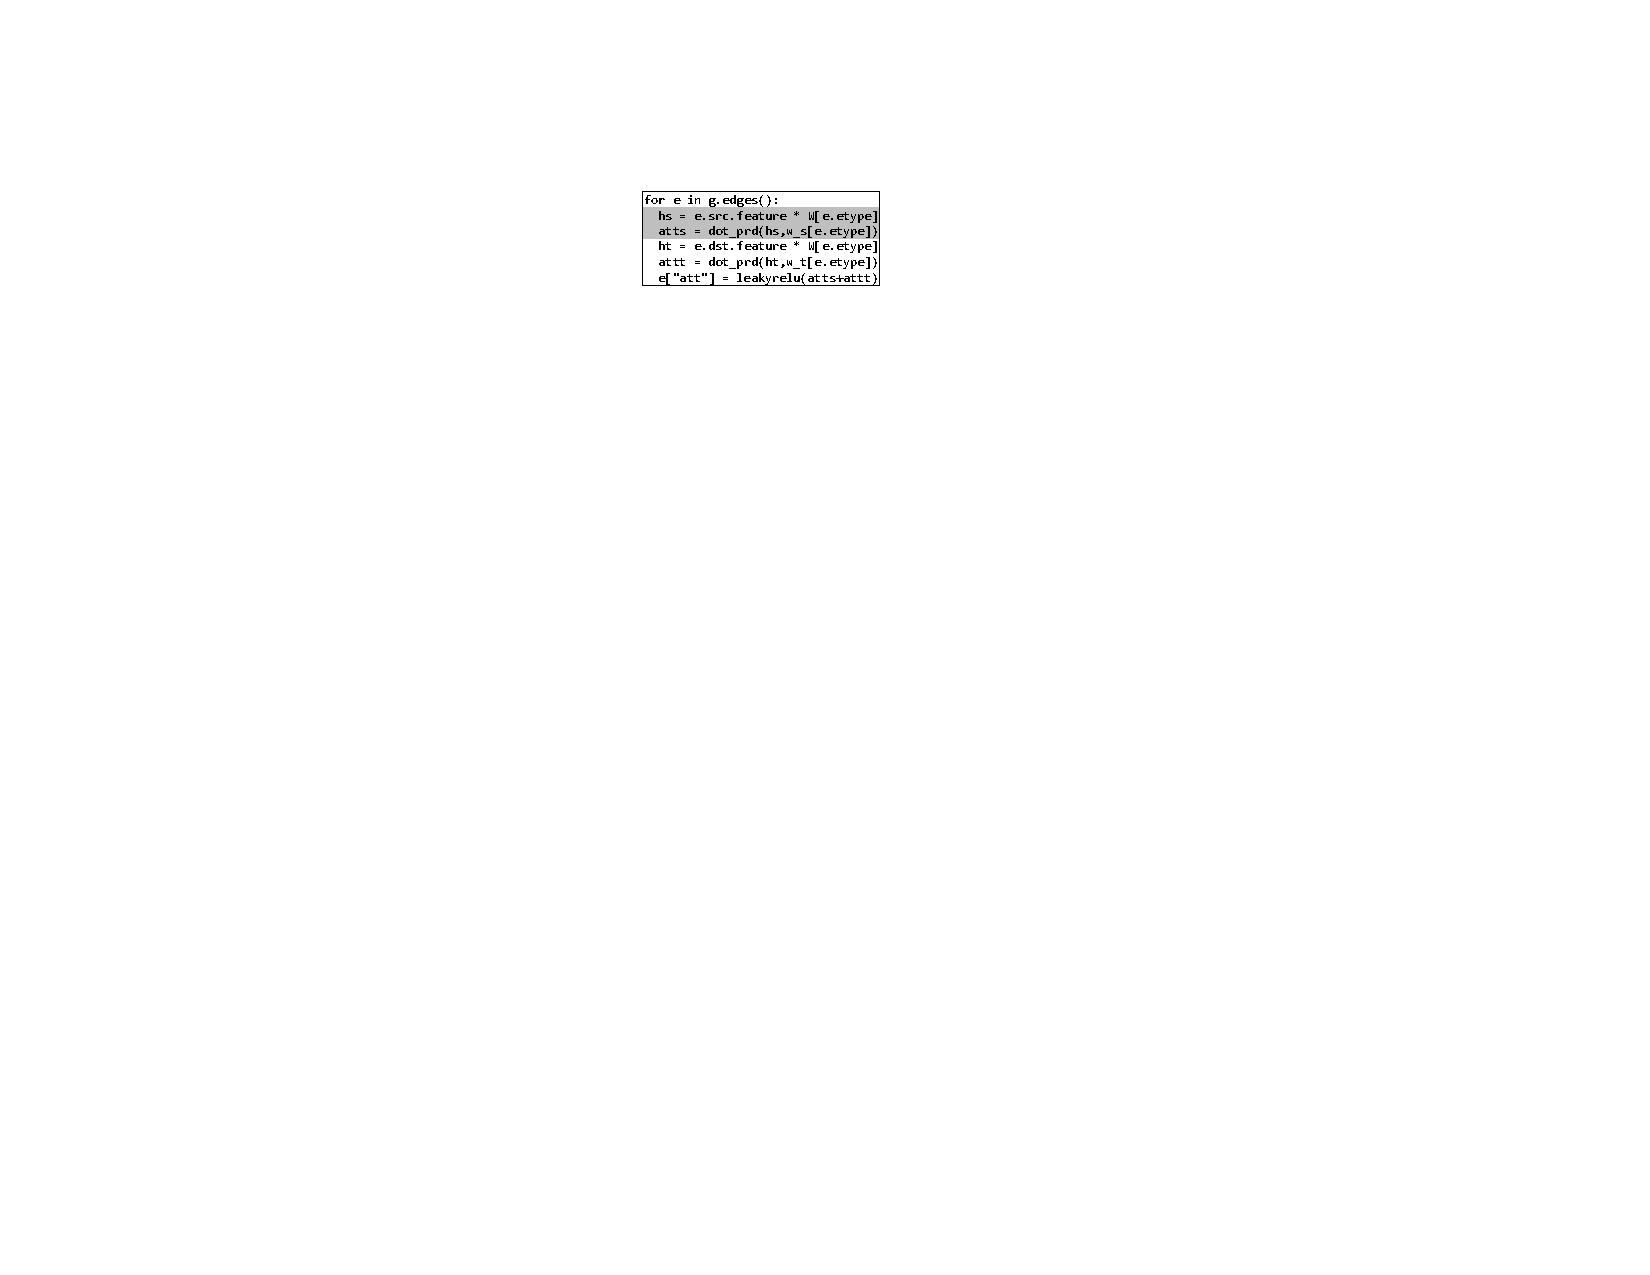
\includegraphics[scale=1.8]{figures/Hector/supplemental_linear_opt.final.1.pdf}}
\subcaptionbox{After the linear operator reorder, the gray region in (a) is rewritten.}
[\linewidth]{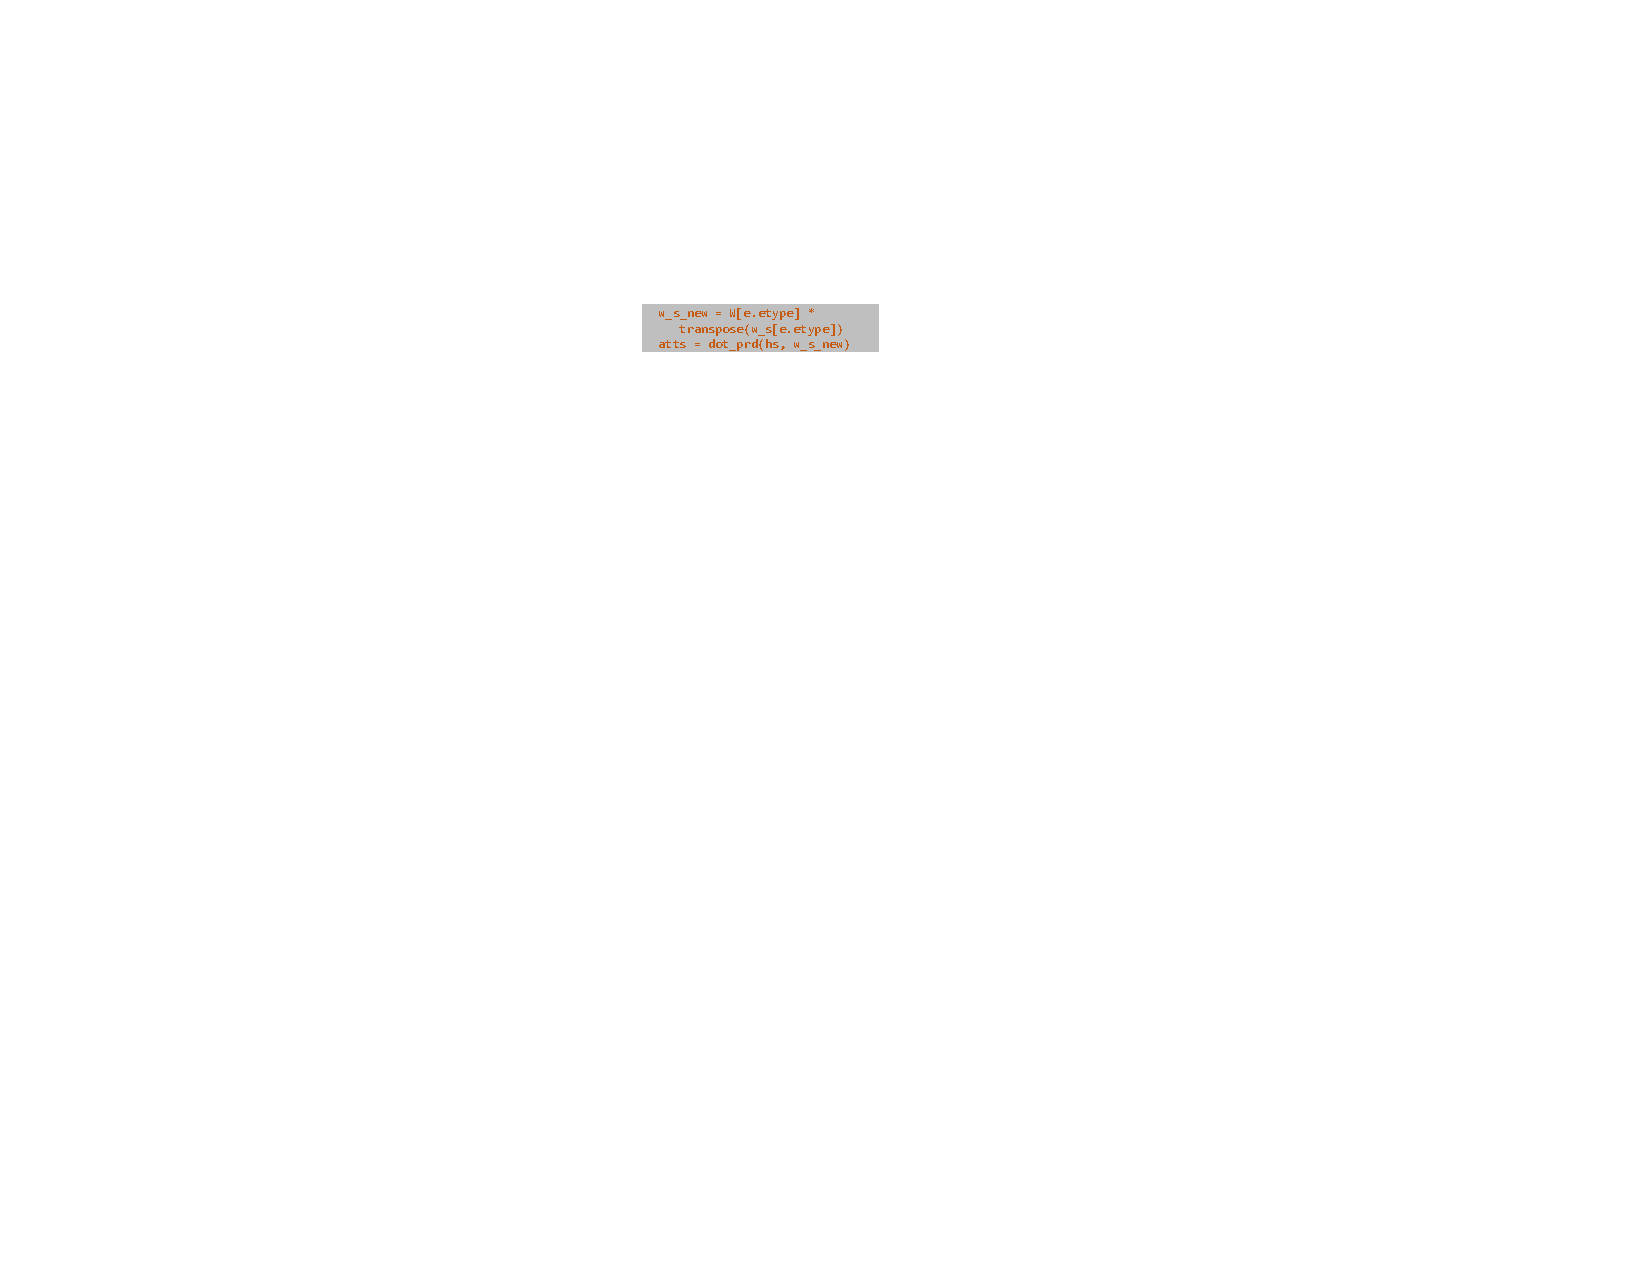
\includegraphics[scale=1.8]{figures/Hector/supplemental_linear_opt.final.2.pdf}}
\subcaptionbox{Visualization of computing \texttt{atts} in (a). Orange parentheses mark the computation order change after linear operator reorder.}
[\linewidth]{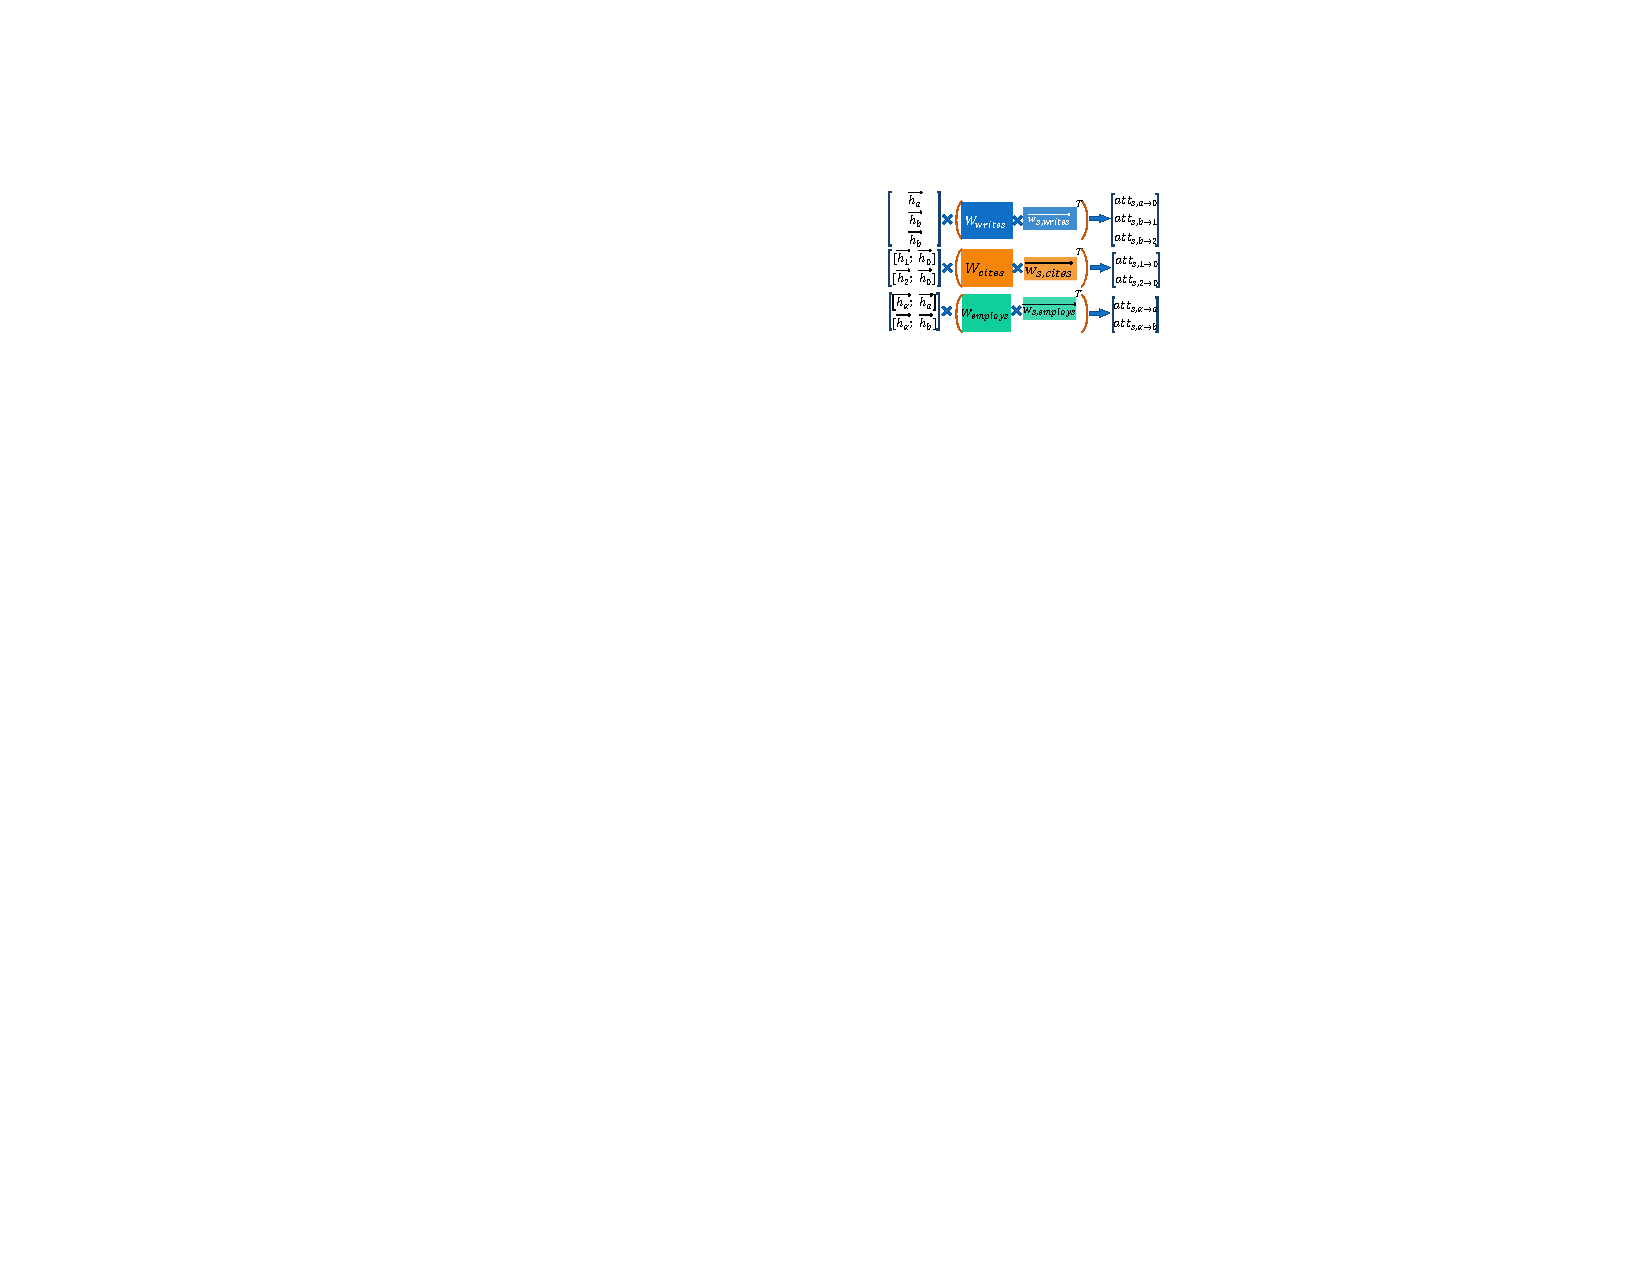
\includegraphics[scale=1.8]{figures/Hector/supplemental_linear_opt.final.3.pdf}}
\caption{\label{fig:linear_opt} In the example graph in Figure~\ref{fig:opt_example}, when computing edge attention of RGAT, linear operator reordering could be applied. (a) shows the original inter-operator level IR to compute RGAT edge attention. (c) visualizes the computation of the first term, \texttt{atts}, and uses the orange parentheses to mark how the linear operator reordering changes the order of the computation. (b) The transformation rewrites the code.}
\end{figure}





\subsubsection{Graph-Semantic-Aware Loop Transformation}\label{sec:graph_aware_loop}
Loop transformation at this level is augmented with the graph-semantic-specific equivalence rule: a for-each loop over the edges is equivalent to a for-each loop nest iterating over all the incoming/outgoing edges of all destination or source node. Loop transformation is applied during the lowering pass to canonicalize and fuse loops in order to more thoroughly identify kernel fusion opportunities. 


\subsubsection{Lowering Inter-Operator Level IR}

To lower the IR to the intra-operator level, Hector greedily lowers every eligible operator to instances derived from GEMM templates~(Section~\ref{sec:two_templates}). Then, it fuses each remaining region and lower them to as few traversal instances~(Section~\ref{sec:two_templates}) as possible.
To achieve this, Hector scans the code three times. Each time, it attempts to lower operators to instances of a specific preference level. During the first pass, it attempts to lower operators to GEMM-template-derived instances. In the next pass, it attempts the traversal-template-derived instances. The third pass will lower all the remaining operators to PyTorch function calls.
During each pass, whenever an operator can be lowered, Hector marks the operator itself, together with all subsequent operators that can be fused into it, with the lowering decision. 
After all the operators have been examined in a pass, the marked operators are lowered and fused. Before the second pass, it canonicalizes the for loops and fuses loop nests whenever possible to discover kernel fusion opportunities. 







\subsection{Intra-Operator Level IR}\label{sec:intra-op-ir}


{The} intra-operator level IR serves between the inter-operator level IR and the generated CUDA code. At this level, the IR should encode specifications to emit CUDA code and provide sufficient information specific to each operator invocation to the transform and lowering passes at the inter-operator level. 
The code transformation components at this level provide the methods to generate specialized CUDA code for the operators, to apply operator-specific schedules, and to return necessary information on operator selection and kernel fusion feasibility to the passes at the inter-operator level.

Hector's code generator ultimately lowers the IR to two basic constructs, the GEMM template and the traversal template. 
Algorithms~\ref{algo:gemm_template} and~\ref{algo:traversal_template} illustrate the edge traversal template and the GEMM template. 
The node traversal template is similar to Algorithm~\ref{algo:traversal_template}, and we will revisit it in Section~\ref{sec:op_schedule}.
For simplicity, function template specialization refers to routines specialized for the specific instances derived from the two templates and involve 1)~function arguments, e.g., number of rows, etc., 2)~special registers, e.g., \texttt{threadIdx}, and 3)~loop variables.







\subsubsection{The GEMM Template and the Traversal Template}\label{sec:two_templates}
We base the code generation on GEMM and traversal templates because RGNNs involve not only sparse operations but also multiple dense operations to project vectors across different semantic spaces.
The GEMM template serves edgewise and nodewise linear transformations, as exemplified by the computation of RGAT edge messages in Figure~\ref{fig:compact_opt_opt}. The GEMM template is defined as a matrix multiply augmented with custom gather and scatter schemes. It is formulated as $Y[S] = X[G] \times W[T]$ where $Y$, $X$, $W$ are output, input, and weights, respectively; $S$, $G$, and $T$ are scatter list, gather list, and the type of the nodes or edges, respectively. 
The traversal template performs generic nodewise or edgewise operations. It serves operators that cannot be lowered to GEMM templates, e.g., edgewise dot products.

As shown in Algorithm~\ref{algo:gemm_template}, the GEMM template is based on tiled matrix multiplication. The GEMM template starts with %
the work assignment per block during the \texttt{GetRange<kid>} subroutine~(line 1). 
The \texttt{idxTileRow} and \texttt{idxTileCol} whose range is determined by \texttt{GetRange<kid>} is used to position the workload.
Typically, it is the coordinate of the tile of the output matrix.
Factors that affect $X$'s loading scheme, \texttt{LoadXToShmemIfInRange<kid>}, and $W$'s, \texttt{LoadWToShmemOrRegistersIfInRange<kid>}, involve whether gather lists or transpose needs to be applied on the fly~(lines 4-5).
Gather list $G$ in the Input section is sometimes needed to locate the rows in the source matrix $X$: For example, in Figure~\ref{fig:compact_opt_opt}(a), \texttt{row\_idx} is needed in step \textcircled{1}.
The required information will be passed during the lowering.
The operator instance then accordingly chooses the data access scheme code piece for kernel code generation.
The storing scheme \texttt{StoreCIfInRange<kid>} depends similarly on whether a scatter list will be applied. 
Atomic intrinsics are used in the case of multiple simultaneous updaters.




In the traversal template, as shown in
Algorithm~\ref{algo:traversal_template}, the edge type, node indices retrieval scheme in lines~5-7 depend on the sparse adjacency encoding.
Similarly to the GEMM template, when a row vector needs to be loaded or stored, the tensor materialization scheme determines how the row is located in the materialized tensor.
All statements are initially inserted into the innermost loop. 
After Hector finishes the loop transformations, it then defines work assignment on line~1 in Algorithm~\ref{algo:traversal_template} for the operator instance derived from the traversal template using a simple scheme. For example, if the loop nest is three levels, as exemplified by Algorithm~\ref{algo:traversal_template}, we assign the outermost loop, i.e., \texttt{idxEdge} or \texttt{idxNode} loop, to each thread block and the two inner loops to the multi-dimensional threads in each block.


\begin{algorithm}[!htbp]
{
\KwIn{References of Tensor $Y, X, W$, gather list $G$, etc.}
\texttt{tileRowRange}, \texttt{tileColRange} $\gets$ \textbf{\texttt{GetRange<kid>}}()\;
\ForEach{\texttt{idxTileRow} $\in$ \texttt{tileRowRange}}{
\ForEach{\texttt{idxTileCol} $\in$ \texttt{tileColRange}}{
\textbf{\texttt{LoadXToShmemIfInRange<kid>}}()\;
\textbf{\texttt{LoadWToShmemOrRegistersIfInRange<kid>}}()\;
\texttt{\_\_syncthreads()\;}
\texttt{Y\_reg} $\gets$ \texttt{X\_shmem} $\times$ \texttt{W\_shmem\_or\_reg}\;
\texttt{\_\_syncthreads();}
}
\textbf{\texttt{StoreYIfInRange<kid>}}()\;
}
}
\caption{Hector's GEMM template in pseudo-code. Each instance is assigned a unique identifier \texttt{kid} and gets function template specialization \textbf{\texttt{FuncName<kid>}}.}
\label{algo:gemm_template}
\end{algorithm}


\begin{algorithm}[!htbp]
{
\KwIn{References of input and output tensors. Other necessary data, e.g., adjacency.}
\texttt{eRange}, \texttt{hRange}, \texttt{fRange} $\gets$ \textbf{\texttt{GetRange<kid>}}()\;
\ForEach{\texttt{idxEdge} $\in$ \texttt{eRange}} {
    \ForEach{\texttt{idxHead} $\in$ \texttt{hRange}}{
        \ForEach{\texttt{idxFeat} $\in$ \texttt{fRange}}{
        \texttt{eType} $\gets$ \textbf{\texttt{GetEType<kid>}}()\;
        \texttt{srcIdx} $\gets$ \textbf{\texttt{GetSrcId<kid>}}()\;
        \texttt{dstIdx} $\gets$ \textbf{\texttt{GetDstId<kid>}}()\;
        \tcp{initial insertion point}
        }
    }
}
}
\caption{Hector's edge traversal template in pseudo-code. Similarly to Algorithm~\ref{algo:gemm_template}, each instance gets specialized \textbf{\texttt{FuncName<kid>}}.}
\label{algo:traversal_template}
\end{algorithm}


\subsubsection{Adapting to Different Sparse Adjacency Encoding}
At the intra-operator level, the templates work for any sparse adjacency encoding as long as specific interfaces are implemented. For example, the edge traversal shown in Algorithm~\ref{algo:traversal_template} works as long as the function template specialization \texttt{GetEType<kid>}, \texttt{GetSrcId<kid>}, and \texttt{GetDstId<kid>} are implemented: If the sparse adjacency is COO, \texttt{GetSrcId<kid>} is a subscript operator applied to the row indices array. If it is CSR, then \texttt{GetSrcId<kid>} is a binary search in the row pointer array.

\subsection{Rationale of the Hector Two-Level IR}
\label{sec:ir_design}

Central to the code generator is the two-level IR.
Inter-operator level IR optimizations address the opportunities brought in by heterogeneous relation types. These optimizations manipulate operators and their connections. A high-level IR %
abstracts away the low-level details that can complicate or even hinder the transformations. 
Intra-operator level IR optimizations reduce the data movement by generating access schemes in kernels rather than using specialized kernels and dedicated indexing/copying kernels. These optimizations manipulate low-level data access and schedule details, and thus are better supported by a low-level IR.


The two-level IR enables concerted but decoupled choices of intermediate data layout and compute schedules.
For example, in Figure~\ref{fig:runtime_arch}, the semantics of the model are decoupled from the layout choices.
Hector implements the model semantics and layout choices in intra-operator level IR with specific access schemes.
The next few paragraphs explain how the two-level IR design facilitates operator-specific optimizations, operator selection, and kernel fusion.

\subsubsection{Operator-Specific Schedule}
\label{sec:op_schedule}
Each instance derived from the GEMM template provides the option to apply a coarsening factor in $\{2,4\}$, to choose the tile size, and to apply \texttt{\_\_launch\_bounds\_\_} that limits the number of registers in exchange for more active warps. 
The coarsening factor is the number of elements each thread deals with in the loading, computing, and storing stages. When applied, each block still works on the same assignment, but its number of threads shrinks by the factor~\cite{PMPP4}.
We also allow a per-row scalar to be applied to the tiles of matrix $A$.
This eliminates the extra memory-intensive traversal to perform weighted vector summation by attention or norm.

As for the traversal template, similarly to the discussion in Section~\ref{sec:graph_aware_loop}, we incorporate graph-semantic-aware loop transformation rules that allow Hector to leverage graph semantics to open up the trade-off between more data reuse opportunities and greater parallelism. As mentioned in Section~\ref{sec:two_templates}, initially, all statements are in the innermost loop in each instance derived from the traversal template. 
Loop hoisting is performed to enhance data reuse: The template features insertion points before and after the end of each loop level. For each statement, Hector finds the outermost level where it can be placed before applying the template. 
In addition, the template also provides a partial result aggregation method, which is applied during lowering by default, to reduce global memory traffic by accumulating results within a thread and within a warp before atomically adding them to the data in global memory.


\subsubsection{Operator Selection and Kernel Fusion}
Transformation and lowering passes at the inter-operator level need information about operator instances, specifically operator preference %
and the feasibility of kernel fusion.
Preference level is the mechanism Hector uses to select the operator instance when there are multiple candidates. For example, an operator instance derived from the GEMM template may %
 have an alternative derived from the traversal template but the alternative would lead to lower performance due to much lower data reuse. 
For good performance, operator instances derived from the GEMM template are assigned a higher preference level than those derived from the traversal template unless otherwise specified. Instances that fall back to PyTorch have the lowest preference level.

Operator instances also provide methods to determine the feasible operators to be fused within the IR. %
Operator instances derived from the GEMM template can be fused with the consumer if 1)~the latter multiplies the row vectors in the GEMM output with scalars and 2)~the two operators are in the same loop~(nest). Operator instances derived from the traversal template can be fused with each other as long as they are in the same loop~(nest).
If the inter-operator level pass finds that some temporary variables are created and merely used inside the fused operator, it passes that knowledge to the method so that the variable no longer needs to be created in the global memory.



\subsection{Backward Propagation}
\label{sec:bck_prop}


Similarly to PyTorch, Hector supports auto-differentiation by %
maintaining the backward propagation counterparts of the operators.
Hector first emits the backward propagation via inter-operator level IR and removes unused gradients and their computation.
The lowering and code generation schemes are similar to those in forward propagation.
However, additional processing is needed because the PyTorch auto-differentiation requires the backward propagation methods to be paired with the forward propagation methods in the \texttt{autograd.Function} definitions. To achieve this, Hector bookkeeps the kernel calls in each forward propagation method. For each forward propagation method, Hector puts all the corresponding backward propagation kernel calls in the body of the backward propagation method.


\subsection{Code Generation}
\label{sec:code_gen}
The code generation procedure emits code based on the CUDA kernel specifications detailed in the form of intra-operator IR. Kernel code generation is fairly straightforward and is implemented using a template-based approach. 
Hector then emits the host functions that configure grids and blocks, gets raw pointers from the \texttt{libtorch} \texttt{at::Tensor} references, and launches the corresponding kernel. The host functions are exported via \texttt{pybind11} utilities. 

The Hector performs a pass that scans all the functions generated to collect a list of preprocessing required for the input dataset, involving transposition, converting COO to CSR, etc. The code generator then emits the preprocessing code.


\subsection{Applicability of the Optimizations to GNNs.}\label{sec:gnn_applicability}
Linear operator reordering and compact materialization are specific to RGNNs. Linear operator reordering is specific to RGNNs because RGNNs typically require linear projections from different semantic spaces, introduced by the heterogeneity of node types and edge types, to a common space before further operations. 
Compact materialization is specific to RGNNs because of the additional tensor dimension brought in by different node types and edge types. 

Some of the intra-operator IR optimizations could benefit ordinary GNNs, which can be treated as a special case of RGNNs whose relation type number is one. Intra-operator level IR allows specification of both data access schemes and schedules, thus allowing flexible code generation to accommodate different dense or sparse tensor layouts, a need that often arises from compact materialization. However, the ability to generate code for different data access schemes and schedules can be beneficial when compiling ordinary GNNs.
